Šioje dalyje bus bandoma parodyti, jog reaktyvų programavimą galima panaudoti įvykių kaupimo sistemose. Pirmiausia nagrinėjami jau esantys reaktyvaus programavimo bei įvykių kaupimo programavimo karkasai/bibliotekos. Kad būtų galima susidaryti bendrą vaizdą ir suvokti įvykių kaupimo sistemas, pirmiausia projektuojamas pavyzdinis įvykių kaupimo sistemos architektūros modelis. Toliau aprašomos šio pavyzdinio architektūros modelio komponentų žemesnio lygmens realizacijos detalės, kūrimo gairės. Atsižvelgiant į DDD, prieš pateikiant konkrečius pavyzdžius, skaitytojas yra supažindinamas su domeno sritimi bei galimais įvykiais. Sekančiame poskyryje aprašomas alternatyvus būdas kurti skaitymo modelį pritaikant reaktyvaus programavimo principus ir paslepiant operacijų su duomenų saugykla realizacijos detales.

\subsection{Programavimo kalba}

Pasirinkta griežtai tipizuota, dinaminė ``Ruby'' kalba, palaikanti tiek objektinį, tiek funkcinį programavimą. Kalba yra viena populiariausių atviro kodo talpykloje ``Github'', plačiai naudojama informacinių technologijų industrijoje (``Github'', ``AirBnb'', ``Etsy'', ``Shopify''), lengvai skaitoma, turi daugybę kokybiškų bibliotekų bei atitinka darbo tiksle išsikeltą sąlygą.

\subsection{Reaktyvus programavimas Ruby kalboje}

Žemesniame lygyje paradigma iš esmės yra dviejų kūrimo šablonų konstrukcija, naudojama jau daugiau nei 20 metų. Faktiškai viena iš populiariausių kūrimo šablonų knygų yra „Gang of Four“, kurioje aprašyti šie du kūrimo šablonai: iteratoriaus ir stebėtojo šablonai \cite{GOF:DesignPattern}. Tai yra du elgsenos kūrimo šablonai, charakterizuojantys objektų ir klasių sąveiką ir atsakomybę.

\subsubsection{Iteratorius}

Pagrindinė šio šablono (iteratoriaus) idėja – atsakomybė už sąrašo objekto prieigą ir perėjimą. Iteratoriaus klasė apibrėžia prieigos prie sąrašo elementų sąsają. Iteratoriaus objektas atsakingas už esamo elemento stebėjimą; t. y. jis žino, kurie elementai jau buvo pereiti.

„Ruby“ programavimo kalboje \lstinline|Enumerable| modulis kaip tik tai ir daro: pateikia surašytuvą, kuriame yra uždari duomenys ir perėjimo metodai. Parašykime trumpiau: „Ruby“ iteratorius – tai klasės, į kurią įtrauktas \lstinline|Enumerable| modulis, egzempliorius, kuris yra beveik bet koks rinkinys.

\subsubsection{Stebėtojas}

Stebėtojo šablonas yra kūrimo šablonas, kuriame objektas (vadinamas tema) tvarko jo priklausinių (vadinamų stebėtojais) sąrašą ir automatiškai praneša apie bet kokius būsenos pasikeitimus, paprastai iškviesdamas vieną iš jų metodų. Paprastai jis naudojamas paskirstytųjų įvykių tvarkymo sistemoms realizuoti.

Iš esmės temos yra objektai, kurie siunčia pranešimus į objektus, stebinčius tokias temas. Temos priverstinai įkelia pranešimus stebėtojams, todėl tai ir vadinama stebėtojo šablonu.

„Ruby“ programavimo kalba turi \lstinline|Observable| modulį standartinėje bibliotekoje, kurioje pateikiamas paprastas mechanizmas, skirtas vienam objektui (temai) informuoti prenumeratorių rinkinį (stebėtojus) apie bet kokį būsenos pasikeitimą.

\subsubsection{Reaktyvaus programavimo bibliotekos}

Darbo autoriui pavyko rasti 2 reaktyvaus programavimo bibliotekas ``Ruby'' kalboje, todėl jos bus plačiau aptartos.

\begin{itemize}
  \item ``RxRuby''\footnote{https://github.com/ReactiveX/RxRuby} - 595 žvaigždutės bei 52 išsišakojimai, paskutinis atnaujinimas įvyko 2017 metų sausį. (Žiūrėta 2017-01-08)

  \item ``Frappuccino''\footnote{https://github.com/steveklabnik/frappuccino} - 370 žvaigždučių bei 32 išsišakojimai, paskutinis atnaujinimas įvyko 2016 metų vasarį. (Žiūrėta 2017-01-08)
\end{itemize}

``RxRuby'' biblioteka turi labiau apribojančią ``Apache'' licenziją (2 versija) lyginant su ``Frappuccino'' MIT licenzija.

\subsubsection{RxRuby}

Pirmiausia pažiūrėkime kaip veikia ``RxRuby'' paprasčiausioje formoje:

\begin{lstlisting}[]
  RxRuby::Observable.just(7)
\end{lstlisting}

\lstinline|RxRuby::Observable| yra srautas. Srautas yra tema (arba objektas), kurį galima prenumeruoti (arba stebėti). \lstinline|RxRuby::Observable| modulis pats nedaro nieko, nebent kuris nors jo metodas bus iškviestas. Tęskime pavyzdį:

\begin{lstlisting}[]
  stream = RxRuby::Observable.just(7)
  stream.subscribe { |num| puts "Gautas skaicius #{num}" }
\end{lstlisting}

Objektas, kurį gauname, yra tiesiog skaičius 7, apgaubtas kaip tema. Kadangi tema realizuoja daugumą \lstinline|Enumerable| modulio metodų, galima su juo daryti praktiškai bet ką. Tačiau, kad išvengtume sudėtingumo šiame pavyzdyje, tiesiog prenumeruokime temą ir perduokime \lstinline|lambda| konstrukciją. \lstinline|Lambda| bus iškviesta kiekvieną kartą, kai srautas gaus informaciją (šiuo atveju tik kartą).

Šio pavyzdinio atvejo išvestis bus:

\begin{lstlisting}[]
  Gautas skaicius 7
\end{lstlisting}

Kadangi turime daug \lstinline|Enumerable| modulio metodų, kuriuos galime naudoti, galime kažką nuveikti su masyvu. Yra 2 būdai dirbti su masyvais ``RxRuby'' bibliotekoje: naudojant rėžį ir paprastus masyvus.

\begin{lstlisting}[]
  RxRuby::Observable.range(1,10)
    .select { |num| num.even? }
    .sum
    .subscribe { |s| puts "Suma lyginiu skaiciu tarp 1 ir 10 yra: #{s}" }
\end{lstlisting}

Grąžins:

\begin{lstlisting}[]
  Suma lyginiu skaiciu tarp 1 ir 10 yra: 30
\end{lstlisting}

Paanalizuokime šį pavyzdį. Pirmiausia sukuriamas temos rėžis, su skaičiais tarp 1 ir 10. Tada iškviečiamas filtravimo operatorius \lstinline|select| temai, perduodant \lstinline|lambda| kaip parametrą. \lstinline|lambda| priima kiekvieną rėžio skaičių kaip parametrą ir filtruoja visus lyginius temos skaičius, grąžindama naują temą. Iškvietus \lstinline|sum| operatorių, susumuojami visi lyginiai skaičiai.

Galiausiai operatoriaus \lstinline|sum| grąžinama tema yra prenumeruojama. Prenumeruojant tema (arba duomenų srautas) tiesiog stebima ir \lstinline|lambda| iškviečiama. Kiekvieną kartą, kai tema gauna naują informaciją, duomenys perduodami lyg per ``piltuvėlį'' ir paskutinė \lstinline|lambda| atspausdina rezultatą.

\subsubsection{Frappuccino}

Steve Klabnik, žymus žmogus Ruby bendruomenėje dėl savo įnašo į atviro kodo projektus\footnote{https://github.com/steveklabnik}, 2013 metais pristatė reaktyvaus programavimo idėjas Ruby kalboje įvairiose konferencijose, tarp jų Euruko2013 \cite{klabnik:euruko}, RubyConf India 2013 \cite{klabnik:india} ir kitos.

Panagrinėkime ``Frappuccino'' bibliotekos panaudojimo pavyzdį, pavaizduotą \ref{frappuccino} kodo pavyzdyje:

\begin{lstlisting}[caption=``Frappuccino'' bibliotekos panaudojimo pavyzdys, label=frappuccino]
class Button
  def push
    emit(:pushed) # emit sends a value into the stream
  end
end

button = Button.new
stream = Frappuccino::Stream.new(button)

counter = stream
            .map { |event| event == :pushed ? 1 : 0 } # convert events to ints
            .inject(0) { |sum, n| sum + n } # add them up

counter.now # => 0

button.push
button.push
button.push

counter.now # => 3

button.push

counter.now # => 4
\end{lstlisting}

Ši biblioteka, kaip ir RxRuby, naudoja stebėtojo projektavimo šabloną. Sukuriant srautą, klasė \lstinline|Button| iš tikrųjų dinamiškai išplečia \lstinline|Frappuccino::Source| klasę, kuri turi \lstinline|emit| metodą. Taipogi \lstinline|Button| klasė paverčiama tema. \lstinline|emit| metodas iškviečia \lstinline|notify_observers(value)| metodą ir nauja reikšmė perduodama visiems stebėtojams.

Reaktyūs operatoriai (tokie kaip \lstinline|map|, \lstinline|merge| ir kiti) yra realizuoti grąžinant naują \lstinline|Frappuccino::Stream| objektą, kuris taip pat yra stebėtojas.

Šiame pavyzdyje yra sukuriamas mygtukas. Kiekvieną kartą, kai jis paspaudžiamas, visiems temos stebėtojams yra perduodamas pranešimas apie naują reikšmę. \lstinline|counter| kintamasis parodo, kiek kartų buvo paspaustas mygtukas. Nereikia kaskart iš naujo pritaikyti skaičiavimų, biblioteka leidžia apsirašyti elgseną vieną kartą deklaratyviai. \lstinline|map| reaktyvus operatorius transformuoja įvykio reikšmę - jeigu gautas simbolis \lstinline|:pushed| - reikšmė tampa 1, o priešingu atveju 0. Kitas operatorius \lstinline|inject| priima parametrą - pradinę reikšmę (šiuo atveju 0). Kiekvieną kartą, kai yra gaunama reikšmė, perduodamas kodo blokas (\lstinline|lambda|) yra iškviečiamas ir rezultatas atnaujinamas.

Rezultatas yra saugomas atmintyje, todėl programai baigus darbą, reikšmės yra prarandamos. Pranešimo metu tarptautinėje konferencijoje ``Euruko'' Steve Klabnik pasakojo, kad tokią biblioteką būtų galima naudoti vartotojo sąsajos programose. Jis teigia, jog pati idėja yra pasiskolinta iš funkcinių programavimo kalbų, ir įdomu pritaikyti naujus principus Ruby programavimo kalboje.

Kadangi reaktyvūs operatoriai grąžina naują stebėtoją - galima programuoti labai deklaratyviai:

\begin{lstlisting}
  merged_stream = Frappuccino::Stream.merge(one_stream , other_stream)
  filtered_stream = merged_stream.select{ |event| event == :pushed }

  filtered_stream.on_value do |event|
    # event will only ever be :pushed
  end
\end{lstlisting}

Biblioteka leidžia tiek apjungti, tiek filtruoti, tiek perduoti bloką kodo, kuris bus įvykdomas, kai tik srautas gaus naują informaciją.

\subsection{Įvykių kaupimas Ruby kalboje}

Įvykių kaupimo principą taikančių bibliotekų Ruby kalboje nėra daug. Galima būtų išskirti 3 žinomiausias:

\begin{itemize}
  \item ``RailsEventStore''\footnote{https://github.com/arkency/rails\_event\_store} - 212 žvaigždučių bei 18 išsišakojimų, paskutinis atnaujinimas įvyko 2016 metų gruodį. (Žiūrėta 2017-01-07)

  \item ``Sandthorn''\footnote{https://github.com/Sandthorn/sandthorn} - 110 žvaigždučių bei 4 išsišakojimai, paskutinis atnaujinimas įvyko 2016 metų balandį. (Žiūrėta 2017-01-07)

  \item ``Event Sourced Record''\footnote{https://github.com/fhwang/event\_sourced\_record} - 31 žvaigždutė bei 5 išsišakojimai, paskutinis atnaujinimas įvyko 2015 metų balandį. (Žiūrėta 2017-01-07)
\end{itemize}

Visos bibliotekos turi MIT licenziją. Verta paminėti, jog ``RailsEventStore'' anksčiau turėjo labiau apribojančią LGPLv3\footnote{https://github.com/arkency/rails\_event\_store/commit/212b202f227a98f131dc3e8711e431e1f126b475} licenziją (iki 2016 metų birželio).

Kadangi ``RailsEventStore'' yra aktyviai atnaujinima, populiariausia iš trijų, atviro kodo, įvykių kaupimą įgyvendinanti biblioteka, ją ir nagrinėsime.

\subsubsection{RailsEventStore}

Įvykių kaupimo biblioteka ``RailsEventStore'' naudoja atskirą biblioteką darbui su įvykiais pavadinimu ``rails\_event\_store\_active\_record''\footnote{https://github.com/arkency/rails\_event\_store\_active\_record}. Pagal nutylėjimą ji yra numatytoji, tačiau esant reikalui lengvai pakeičiama (pavyzdžiui, norint naudoti Greg Young ``GetEventStore''\footnote{https://geteventstore.com/} duomenų saugyklą). Taip pat yra galimybė naudoti duomenų saugyklą atmintyje.

\subsubsection{Naudojimas}

Kai į ``Ruby on Rails'' projekto \lstinline|Gemfile| failą jau įtrauktas \lstinline|rails_event_store| modulis, reikia sugeneruoti aktyvaus įrašo migraciją:

\begin{lstlisting}[]
  rails generate rails_event_store:migrate
  rake db:migrate
\end{lstlisting}

Sukurta migracija pavaizduota \ref{event_store_events_table} kodo pavyzdyje. Matome, jog kiekvienas įvykis turi srauto pavadinimą, įvykio tipą, unikalų identifikatorių, tam tikrus meta duomenis (čia gali būti tokia informacija kaip kliento IP, šalis iš kurios buvo atlikta užklausa ir t.t.), duomenų laukas, kuris aktyvaus įrašo pagalba serializuojamas į maišos duomenų struktūrą (angl. hash) bei sukūrimo laiką. Taipogi sukuriami reikalingi indeksai, kurie reikalingi greitesnėms užklausoms filtruojant pagal indeksuojamus lentelės stulpelius.

\begin{lstlisting}[caption=Įvykių saugojimo migracija, label=event_store_events_table]
    create_table(:event_store_events) do |t|
      t.string      :stream,      null: false
      t.string      :event_type,  null: false
      t.string      :event_id,    null: false
      t.text        :metadata
      t.text        :data,        null: false
      t.datetime    :created_at,  null: false
    end
    add_index :event_store_events, :stream
    add_index :event_store_events, :created_at
    add_index :event_store_events, :event_type
    add_index :event_store_events, :event_id, unique: true
\end{lstlisting}

Norint naudoti bibliotekos funkcionalumą, tereikia sukurti \lstinline|RailsEventStore::Client| klasės egzempliorių:

\begin{lstlisting}[]

   client = RailsEventStore::Client.new
\end{lstlisting}

\subsubsection{Įvykių kūrimas}

Kurti įvykius naudojantis šia biblioteka yra tikrai paprasta. Tereikia apibrėžti įvykio modelį išplečiant \lstinline{RailsEventStore::Event} klasę:

\begin{lstlisting}[]

  class ProductAdded < RailsEventStore::Event

  end
\end{lstlisting}

Dabar galima sukurti įvykio egzempliorių ir išsaugoti į duomenų bazę:

\begin{lstlisting}[]

  stream_name = "product_1"

  event_data = {data: { name: "Product" }}
  event = ProductAdded.new(event_data)
  # publishing event for specific stream
  client.publish_event(event, stream_name)
  # publishing global event with stream_name == 'all'
  client.publish_event(event)
\end{lstlisting}

Biblioteka suteikia galimybę kurti ne tik specifinius įvykius, bet ir globalius. \lstinline|event_id| yra neprivaloma reikšmė. Jeigu ji neperduodama, biblioteka pati sugeneruoja unikalų identifikatorių.

``RailsEventStore'' biblioteka taip pat turi optimistinę lygiagretumo kontrolę. Galima iš anksto apibrėžti laukiamą srauto versiją bekuriant įvykį. Šiuo atveju tai paskutinio įvykio reikšmė:

\begin{lstlisting}[]

stream_name = "product_1"

  event_data = {

      data: { name: "Product" },

      event_id: "b2e526fd-609d-4ds7-b2df-c624575c8edd"

  }

event = ProductAdded.new(event_data)

  expected_version = "951d352a-a53v-42a1-a5zz-as24chuf5b2l"

client.publish_event(event, stream_name, expected_version)
\end{lstlisting}

\subsubsection{Įvykių skaitymas}

Biblioteka pateikia kelis būdus skaityti įvykius iš duomenų bazės. Visais atvejais įvykiai yra išrūšiuoti didėjančia tvarka.

Galime skaityti tam tikrą skaičių įvykių pradedant tam tikru įvykiu:

\begin{lstlisting}[]
stream_name = "product_1"

start_event = "b2d506fd-409d-4ec7-b02f-c6d2295c7edd"
count = 40
client.read_all_events(stream_name, start_event, count)
\end{lstlisting}

Galime skaityti visus konkretaus srauto įvykius:

\begin{lstlisting}[]
stream_name = "product_1"

client.read_all_events(stream_name)
\end{lstlisting}

Galime skaityti apskritai visus įvykius

\begin{lstlisting}[]
client.read_all_streams
\end{lstlisting}

\subsubsection{Įvykių trynimas}

Įvykių kaupimo principas teigia, jog įvykių žurnalas yra visa sistemos istorija ir įvykiai netrinami. Tačiau gali atsirasti tokia situacija, jog programuotojas dirba lokaliai ir tiesiog testuojasi sistemą ir bando funkcionalumą, nenori užteršti istorijos. Dėl šios priežasties biblioteka palieka galimybę trinti įvykius. Tačiau reiktų gerai pagalvoti prieš naudojant šią komandą.

\begin{lstlisting}
stream_name = "product_1"
client.delete_stream(stream_name)
\end{lstlisting}

\subsubsection{Prenumeratų mechanizmas}

Biblioteka leidžia sinchroniškai klausyti specifinių įvykių. Prenumeratorių mechanizmo panaudojimas demonstruojamas \ref{event_store_subscription} kodo pavyzdyje. Vienintelis reikalavimas yra, jog prenumeratoriaus klasė turi įgyvendinti \lstinline|call(event)| metodą.

Šis funkcionalumas yra įgyvendintas naudojant reaktoriaus projektavimo šabloną (angl. Reactor pattern). Verta pastebėti, jog įvykių srautas gali būti begalinis, apibrėžiama, kas nutikus įvykiui yra įvykdoma, tai yra atnaujima dabartinė prekių krepšelio reikšmė. Prenumeruojami iškart keli įvykių tipai, tai yra 2 skirtingi srautai. Galime šį veikimą laikyti kaip reaktyvaus operatoriaus \lstinline|merge| realizaciją.

\begin{lstlisting}[caption=``EventStore'' bibliotekos prenumeratorių mechanizmo panaudojimas, label=event_store_subscription]
class CartReadModel
    def call(event)
        if event.event_type == 'AddToCart'
            add_to_cart(event.data)
        end
        if event.event_type == 'RemoveFromCart'
            remove_from_cart(event.data)
        end
    end
    private
    def add_to_cart(event_data)
        #Implementation here
    end
    def remove_from_cart(event_data)
        #Implementation here
    end

end


cart = CartReadModel.new
client.subscribe(cart, [AddToCart, RemoveFromCart])

\end{lstlisting}

\subsection{Įprastas būdas kurti įvykių kaupimo sistemas IT industrijoje}

Kad būtų lengviau suprasti įvykių kaupimo sistemas bei jos komponentus, šiame poskyryje sukursime pavyzdinę įvykių kaupimo sistemos architektūros modelį, apjungiantį modelio-kontrolieriaus-vaizdo projektavimo šabloną, komandų-užklausų atskyrimo principą bei įvykių kaupimą. Šiame poskyryje bus demonstruojama kaip įprasta kurti tokias sistemas informacinių technologijų industrijoje bei bus gilinamąsi į kiekvieną komponentą žemesniame, kodo lygmenyje.

\subsubsection{Pavyzdinė įvykių kaupimo sistemos architektūra}

Tarkime turime tipinę saityno serverio sistemą, paremtą modelio-vaizdo-kontrolieriaus (MVC) projektavimo šablonu, kurį dar 9 dešimtmetyje aprašė Glenn Krasner ir Stephen Pope kaip bendrinę sąvoką \cite{Krasner:1988:CUM:50757.50759}.

\ref{img:mvc_cqrs} paveikslėlyje pavaizduotas architektūros modelis naudojant MVC projektavimo šabloną bei apjungiantis komandų-užklausų atskyrimo , įvykių kaupimo principus bei reaktyvųjį programavimą. Toliau ši diagrama bus išsamiau paaiškinta bei aprašyta pagrindiniai proceso tėkmės atvejai, komandų operacijos (keičiančios būseną) bei užklausų operacijos (nekeičiančios būsenos).

\begin{figure}[H]
    \centering
    \includegraphics[scale=0.6]{img/mvc_cqrs}
    \caption{MVC paremtas architektūros modelis, apjungiantis CQRS, ES bei reaktyvaus programavimo principus}
    \label{img:mvc_cqrs}
\end{figure}

\textbf{Pavyzdinis procesas - vartotojas įsideda daiktą į pirkinių krepšelį}

\begin{enumerate}
  \item Vartotojas pateikia užklausą programai įdėti pirkinį į pirkinių krepšelį. Pavyzdinė užklausos semantika - \lstinline|https://mysite.com/cart/add/1|.

  \item Saityno serveris gauna užklausą. Maršrutizatorius naudoja maršrutų failą \lstinline|config/routes.rb| ir identifikuoja kur reikia nusiųsti užklausą. Mūsų atveju \lstinline|cart| yra kontrolierius, \lstinline|add| yra norimas atlikti veiksmas, o \lstinline|1| yra parametras, nurodantis konkretų/unikalų pirkinį.

  \item Kontrolierius iškviečia komandą.

  \item Komanda gali patikrinti ar užklausa buvo teisinga. Jei užklausa buvo teisinga, kontrolierius įrašo sėkmingą arba nesėkmingą įvykį į įvykių kaupimo žurnalą. Taipogi komanda gali atlikti tam tikrus šalutinius efekus, tokius kaip elektronių žinučių siuntimas vartotojui.

  \item Kai įvykis įrašomas į įvykių kaupimo žurnalą, reaktyvaus programavimo programos sąsaja (API) reaguoja į įvykį pagal aprašytas taisykles. Taisyklės aprašo ką su tuo įvykiu reikia padaryti, bendru atveju tai dažniausiai yra dabartinės būsenos atnaujinimas tam tikroje kitoje duomenų saugykloje.

  \item Kai tik įvykis jau įrašytas į įvykių žurnalą, galima vartotojui pranešti apie sėkmingą rezultatą.
\end{enumerate}

\textbf{Pavyzdinis procesas - vartotojas peržiūri savo pirkinių krepšelį}

\begin{enumerate}
  \item Vartotojas pateikia užklausą programai peržiūrėti savo pirkinių krepšelį. Pavyzdinė užklausos semantika - \lstinline|https://mysite.com/cart|.

  \item Saityno serveris gauna užklausą. Maršrutizatorius naudojo maršrutų failą \lstinline|config/routes.rb| ir identifikuoka kuris kontrolierius atsakys į užklausą.

  \item Kontrolierius iškviečia skaitymo modelį, kuris naudojant Ruby on Rails karkasą įprastai būna supaprastintas (naudojant aktyvų įrašą nereikia rašyti SQL, jis yra sugeneruojamas). Pavyzdinė užklausa \lstinline|@cart = current_user.cart.all|.

  \item Dabartinis vartotojo pirkinių krepšelis yra nuskaitomas iš duomenų saugyklos. Čia reikia prisiminti galutinės darnos sąvybę. Esant didelei apkrovai, egzistuoja galimybė, jog bus nuskaitoma krepšelio būsena, kai pirkinys dar nepridėtas į krepšelį. Todėl toks sistemos projektavimas verčia labiau mąstyti apie pačią sistemą. Įprastiniu atveju, pirkinių krepšelis įvykdžius daikto pridėjimo scenarijų, aprašytą aukščiau, galėtų būti pridedamas vartotojo sąsajoje. Vartotojas matytų, jog pirkinys pridėtas į krepšelį, tačiau įvykių kaupimo programavimo programos sąsaja (API) dar galbūt nebūtų baigusi darbo. Kai vartotojas norėtų pirkti visus krepšelio pirkinius, reaktyviojo programavimo programos sąsaja (API) jau būtų baigusi darbą. Įprastiniu atveju tai trunka keliasdešimt milisekundžių.

  \item Galiausiai vartotojui pateikiamas krepšelio vaizdas.
\end{enumerate}

\subsubsection{Domeno modelis}

Remiantis literatūros analizėje aptartu domenu pagrįstu projektavimu - pradedant kurti įvykių kaupimo sistemą, pirmiausia reikia apsibrėžti domeno modelį, arba tiksliau agregatus, kuriuos aprašo Martin Fowler \cite{Fowler:Aggregate}. Naudojant įvykių kaupimą, domeno modelis yra sukuriamas remiantis domeno įvykiais. Duomenų struktūra nesaugo dabartinės būsenos, o saugo eilę domeno įvykių, kurie buvo pritaikyti agregatui nuo sistemos gyvavimo pradžios. Tai leidžia konstruoti agregatą, neatskleidžiant jo būsenos ir taip apsaugant jo invariantus.

Agregatas gali būti naujų domeno įvykių šaltinis - kiekvienas agregato metodo kvietimas gali publikuoti naują domeno įvykį. Kiekvienas agregato vidinės būsenos pasikeitimas privalo būti realizuotas publikuojant arba pritaikant domeno įvykį. Tik taip galima užtikrinti, jog taikant įvykius agregatas visada bus atkurtas į tą pačią būseną.

Pirmiausia apsibrėžkime domeno įvykius:

\begin{lstlisting}[]
module Events
  ProductAddedToCart = Class.new(RailsEventStore::Event)
  ProductRemovedFromCart = Class.new(RailsEventStore::Event)
  OrderCreated = Class.new(RailsEventStore::Event)
end
\end{lstlisting}

Pagal nagrinėjamą scenarijų minėti įvykiai apibrėžia šiuos veiksmus:

\begin{itemize}
  \item \lstinline|ProductAddedToCart| - pirkinys pridėtas į krepšelį.
  \item \lstinline|ProductRemovedFromCart| - pirkinys išimtas iš krepšelio.
  \item \lstinline|OrderCreated| - įvykdytas užsakymas.
\end{itemize}

Kai turime apsibrėžtus domeno įvykius, galime juos pritaikyti domeno objektui. Panagrinėkime \ref{apply_domain_events} kodo pavyzdį. \lstinline|Domain::Order| klasė turi metodą \lstinline|initialize|, kuris sukuria pradinę agregato būseną. Taip pat, klasė turi \lstinline|create| metodą. Pastarasis turėtų būti naudojamas kitų objektų, iškviečiant agregato funkcijas. Čia turėtų būti apsaugomi invariantai, tikrinama verslo logika, teisingumo taisyklės. Remiantis CQRS principu, šis metodas neturėtų grąžinti reikšmės - jis privalo būti tik įvykdomas arba nutraukti vykdymą iškeliant išimtinę situaciją. Taipogi šiame metode agregato būsena niekada nėra keičiama. Vietoje to yra sukonstruojamas ir pritaikomas naujas domeno įvykis (kurį apsirašėme anksčiau).

\begin{lstlisting}[caption=Įvykių pritaikymas domeno objektui, label=apply_domain_events]
module Domain
  class Order
    include AggregateRoot::Base

    AlreadyCreated    = Class.new(StandardError)
    MissingCustomer   = Class.new(StandardError)

    def initialize(id = SecureRandom.uuid)
      @id = id
      @state = :draft
    end

    def create(order_number, customer_id)
      raise AlreadyCreated unless state == :draft
      raise MissingCustomer unless customer_id
      apply Events::OrderCreated.create(@id, order_number, customer_id)
    end

    # ...

    def apply_order_created(event)
      @customer_id = event.customer_id
      @number = event.order_number
      @state = :created
    end

    private
    attr_accessor :id, :customer_id, :order_number, :state

    # ...
  end
end
\end{lstlisting}

Reiktų detaliau panagrinėti iš kur įtraukiamas \lstinline|AggregateRoot::Base| modulis. Tai yra ``aggregate\_root''\footnote{https://github.com/arkency/aggregate\_root} biblioteka, kuri atkeliauja kartu su ``RailsEventStore biblioteka''. \ref{aggregate_root} kodo pavyzdyje demonstruojamas svarbiausias funkcionalumas. Modulis įterpia metodą \lstinline|apply|. Kviečiant \lstinline{apply Events::OrderCreated.create(@id, order_number, customer_id)} yra sukuriamas naujas domeno įvykis ir pritaikomas agregatui - būsena pasikeičia ir \lstinline|@unpublished_events| kintamasis saugo pakeitimus. Jis saugo visus agregato sukurtus domeno įvykius, kol metodas yra vykdomas.

Paskutinis svarbus momentas yra \lstinline|apply_order_created| metodas. Pastarasis atnaujina agregato būseną priklausomai nuo įvykusio domeno įvykio. Nesvarbu ar pats agregatas publikavo įvykį, ar įvykis buvo nuskaitytas iš įvykių žurnalo ir pritaikytas atkuriant dabartinę agregato būseną, šioje vietoje negali būti verslo logikos ar teisingumo taisyklių. Tai tik būsenos atkūrimas, o istorijos keisti negalima, kaip buvo nagrinėta literatūroje.

\begin{lstlisting}[caption=``AggregateRoot'' modulis, label=aggregate_root]
module AggregateRoot
  class DefaultApplyStrategy
    def call(aggregate, event)
      event_name_processed = event.class.name.demodulize.underscore
      aggregate.method("apply_#{event_name_processed}").call(event)
    end
  end
end

module AggregateRoot
  def apply(event)
    apply_strategy.(self, event)
    unpublished_events << event
  end

  private

  def unpublished_events
    @unpublished_events ||= []
  end

  def apply_strategy
    DefaultApplyStrategy.new
  end
end
\end{lstlisting}

\subsubsection{Komandos}

Komanda yra paprastas objektas, kuris apibrėžia parametrus veiksmo vykdymui. Remiantis domenu paremtu projektavimu, komanda turėtų būti pavadinta bendrąja verslo kalba (skvarbiąja kalba) ir išreikšti vartotojo ketinimą. Prieš komandos vykdymą turėtų būti užtikrintos teisingumo taisyklės. Teisingumo taisyklės turėtų būti paprastos, pagrįstos pačiais duomenimis, bet ne verslo logika (Kaip jau minėjome praeitame skirsnyje, domeno objektas tikrina verslo logiką).

Pažvelkime į komandos pavyzdį:

\begin{lstlisting}
module Command
  class CreateOrder < Base
    attr_accessor :order_id
    attr_accessor :customer_id

    validates :order_id, presence: true
    validates :customer_id, presence: true

    alias :aggregate_id :order_id
  end
end
\end{lstlisting}

``Ruby'' programavimo kalboje tai dar žinoma kaip formos objektai (angl. Form Objects)\footnote{https://webuild.envato.com/blog/creating-form-objects-with-activemodel-and-virtus/}. Iš esmės, norint leisti patikrinti teisingumo taisykles, tėvinė klasė \lstinline|Base| naudoja dalį \lstinline|ActiveModel| funkcijų:

\begin{lstlisting}
module Command
  class Base
    include ActiveModel::Model
    include ActiveModel::Validations
    include ActiveModel::Conversion

    def initialize(attributes={})
      super
    end

    def validate!
      raise ValidationError, errors unless valid?
    end

    def persisted?
      false
    end
  end
end
\end{lstlisting}

\subsubsection{Komandų apdorojimas}

Komandų doroklė yra pradinis domeno taškas, turintis instrumentuoti domeno objektus ir domeno tarnybas bei vykdyti domeno objektų metodus. Komandų doroklę galima apsirašyti:

\begin{lstlisting}
module Command
  class Handler
    def initialize(repository:, **_)
      @repository = repository
    end

    protected
    def with_aggregate(aggregate_id)
      aggregate = build(aggregate_id)
      yield aggregate
      repository.store(aggregate)
    end

    private
    attr_accessor :repository

    def build(aggregate_id)
      aggregate_class.new(aggregate_id).tap do |aggregate|
        repository.load(aggregate)
      end
    end
  end
end
\end{lstlisting}

Metodas \lstinline|build| ištraukia įvykius iš įvykių saugyklos, naudodamasis agregato unikaliu identifikatoriumi ir paduodamas įvykių srauto vardą. Komandų doroklė iš pradžių atkuria agregato būseną ir tada išsaugo pakeitimus įvykių žurnale. Prisiminkime praeitame skirsnyje aprašytą \lstinline|unpublished_events| kintamąjį. Štai čia atsiskleidžia tikroji jo paskirtis, visi dar nepublikuoti įvykiai yra išsaugomi. Kai įvykis yra išsaugomas, visi prenumeratoriai, kurie stebi ši įvykį (arba temą) yra informuojami apie pasikeitimus.

Taigi išplečiant šį atvejį, galime pavaizduoti užsakymo komandų doroklę:

\begin{lstlisting}
module CommandHandlers
  class CreateOrder < Command::Handler
    def call(command)
      with_aggregate(command.aggregate_id) do |order|
        order.create(command.customer_id)
      end
    end

    private

    def aggregate_class
      Domain::Order
    end
  end
end
\end{lstlisting}

Čia \lstinline|with_aggregate(command.aggregate_id)| metodas grąžina domeno objektą \lstinline|Domain::Order|, atkurtą iš anksčiau sistemoje įvykusių įvykių, kurie skaitomi iš įvykių žurnalo. Tada komandų doroklė iškviečia \lstinline|create| metodą perduodama parametrus, kuriuos gavo iš komandos.

Supratus domeno įvykius, komandas bei komandų doroklę iškyla klausimas: o kaip kontrolierius iškviečia komandą?

Paprastesniam naudojimui galima sukurti atskirą modulį, kurį galima labai paprastai įtraukti į \lstinline|ApplicationController|, jame prirašius \lstinline|include Command::Execute|:

\begin{lstlisting}
module Command
  module Execute
    def execute(command, **args)
      command.validate!
      args = AggregateRoot::Repository.new(event_store) if args.empty?
      handler_for(command).new(**args).call(command)
    end

    private
    def handler_for(command)
      {
        Command::CreateOrder          => CommandHandlers::CreateOrder,
        Command::AddItemToBasket      => CommandHandlers::AddItemToBasket,
        Command::RemoveItemFromBasket => CommandHandlers::RemoveItemFromBasket,
      }.fetch(command.class)
    end
  end
end
\end{lstlisting}

Šiuo atveju iš pradžių yra tikrinamos komandos teisingumo taisyklės. Sukuriamas objektas prieigai prie įvykių žurnalo skaitymo. \lstinline|handler_for| metodas tiesiog aprašo taisykles kuriomis komandos yra priskiriamos jų doroklėms.

Galiausiai iš kontrolieriaus galime sukurti užsakymą:

\begin{lstlisting}
def create
  cmd = Command::CreateOrder.new(order_params)
  execute(cmd)

  redirect_to Order.find_by_uid(cmd.order_id), notice: 'Order was successfully created.'
end
\end{lstlisting}

\subsubsection{Skaitymo modelio kūrimas}

Iki šiol aprašėme kaip vartotojas vykdo komandas, kaip jos apdorojamos, kur įvykdoma domeno logika, kaip publikuojami ir saugomi domeno įvykiai. Prisiminkime, jog domeno objektai neleidžia paimti (arba nerodo) dabartinės būsenos, todėl reikia kito kelio konstruoti duomenis pateikimui vartotojui (vaizde), tai yra skaitymo pusei. Čia verta pažymėti, jog duomenys yra denormalizuoti, jie yra būtent tokie, kokių reikia tam vaizdui paruošti. Šis sprendimas turi didelį našumo privalumą, kai reikalingos labai greitos užklausos, nes nereikia vykdyti sudėtingų užklausų (pvz.: sujungimo). Duomenų saugykla šiuo atveju gali būti bet kokia duomenų bazė tiek reliacinė, tiek grafų ar NoSQL.

Kad galėtume naudotis šiomis greitomis užklausomis, pirmiausia reikia paruošti skaitymo pusės duomenis. Reikia apdoroti įrašytus įvykius ir juos transformuoti į norimą vaizdą.

Taigi galime apsirašyti įvykių kaupimo sistemos maršrutizatorių:

\begin{lstlisting}
module EventStoreSetup
  def event_store
    @event_store ||= RailsEventStore::Client.new.tap do |es|
      es.subscribe(Denormalizers::OrderCreated.new, [Events::OrderCreated])
      es.subscribe(Denormalizers::ProductAddedToCart.new, [Events::ProductAddedToCart])
      es.subscribe(Denormalizers::ProductRemovedFromCart.new, [Events::ProductRemovedFromCart])
    end
  end
end
\end{lstlisting}

Įvykių maršrutizatorius aprašo koks duomenų denormalizatorius apdoroja domeno įvykį arba aibę domeno įvykių. Iš tikrųjų tai ta pati pagrindinė paskirtis kaip ir maršrutizatoriaus MVC projektavimo šablone, kuris pasako kokią užklausą kuris kontrolierius apdoros.

Pažiūrėkime į užsakymo denormalizatoriaus kodą:

\begin{lstlisting}
module Denormalizers
  class OrderCreated
    def call(event)
      return if Order.where(uid: event.data.order_id).exists?
      order = ::Order.new.tap do |o|
        o.uid = event.data.order_id
        o.number = event.data.order_number
        o.customer = Customer.find(event.data.customer_id).name
        o.state = "Created"
      end
      order.save!
    end
  end
end
\end{lstlisting}

Pagrindinė jo paskirtis išsaugoti gautus duomenis į tam tikrus skaitymo duomenų saugyklos stulpelius (ar įrašus - priklausomai nuo duomenų saugyklos tipo). Tačiau atidžiau pažvelkime į šią eilutę - \lstinline|return if Order.where(uid: event.data.order_id).exists?|. Jeigu įvykis jau egzistuoja - jis nėra atnaujinamas. Tai jau tam tikra teisingumo taisyklė, kuri yra patikrinama prieš įrašant duomenis į duomenų saugyklą. Taigi denormalizatorius šiuo atveju turi dvi atsakomybes - filtruoti duomenis ir išsaugoti duomenis į pasirinktą duomenų saugyklą. Kaip pamatysime vėliau darbe, kuriant biblioteką, apjungiančią reaktyvaus programavimo ir įvykių kaupimo principus, skaitymo modelio kūrimas gali būti supaprastintas.

\subsubsection{Skaitymo pusės asinchroninis kūrimas}

Iš tiesų ``RailsEventStore'' biblioteka veikia sinchroniškai, tačiau skaitymo pusę generuoti galima ir asinchroniškai pasitelkiant papildomas bibliotekas tokias kaip ``Sidekiq''\footnote{https://github.com/mperham/sidekiq} ar ``Rescue''\footnote{https://github.com/resque/resque}. Šios bibliotekos pasižymi bendru bruožu - naudoja gijas apdoroti daugybę darbų tuo pačiu metu. Parametrai perduodami šiems darbams dažniausiai saugomi duomenų saugyklose atmintyje, tokiose kaip ``Redis''\footnote{https://redis.io/} ar ``Memcached''\footnote{https://memcached.org/} našumui užtikrinti.

Parodysime kodo pavyzdį kaip atrodytų asinchroninis užsakymo kūrimas panaudojant ``Sidekiq'':

\begin{lstlisting}
module Workers
  class OrderExists
    include Sidekiq::Worker

    def perform(order_id)
      Order.where(uid: order_id).exists?
    end
end

module Filters
  class OrderExists
    def self.execute(event)
      Workers::OrderExists.perform_async(event.data.order_id)
    end
  end
end
\end{lstlisting}

Čia matome, jog darbininko klasėje tereikia pridėti \lstinline|include Sidekiq::Worker| modulį ir įgyvendinti \lstinline|perform| metodą. Įvykdžius \lstinline|Workers::OrderExists.perform_async(event.data.order_id)|, parametrai (unikalus darbo identifikatorius, perduoti parametrai) yra išsaugomi atskiroje duomenų saugykloje (skirtoje būtent tam) į eilę. ``Sidekiq'' procesas tikrina atsiradusius naujus darbus šioje duomenų saugykloje, ir bendru atveju ima juos iš eilės ir priskiria laisvai gijai, kuri apdoroja rezultatą. Esant didesniai sistemos apkrovai yra ganėtinai nesunku pridėti dar vieną serverį, apdorojantį tokius asinchroninius darbus.

Toks asinchroninis darbų apdorojimas padidina sistemos našumą, padaro ją labiau išplečiama, tačiau kaip buvo minėta literatūroje, priverčia atidžiau mąstyti apie pačią sistemą dėl galutinės darnos principo.

Toks būdas gali būti naudingas darbams, kurie užtrunka ilgiau. Pavyzdžiui, sistemoje yra galimybė įkelti prekes ir jų paveikslėlius. Paveikslėlius reikia sumažinti, sukarpyti, suprastinti kokybę ar dar kitaip apdoroti. Toks procesas trunka ilgiau nei paprastas įrašymas į duomenų bazę, todėl iškėlimas būtų labai naudingas didinant sistemos našumą.

\subsection{Reaktyvus programavimas bei įvykių kaupimas kartu}

Šiame poskyryje bus siekiama pasiekti darbo tikslą - pritaikyti reaktyvaus programavimo principus įvykių kaupimo sistemose taip, jog skaitymo modelis būtų kuriamas tik komponavimo būdu, neturėtų būsenos, tai yra visos operacijos su duomenų baze būtų paslėptos. Pirmiausia bus aprašyta problema, su kuria susiduriama kuriant įvykių kaupimo sistemos skaitymo modelį naudojantis ``RailsEventStore'' biblioteka. Vėliau bus pristatyti kuriamos patobulintos bibliotekos reaktyvūs operatoriai bei jų panaudojimo atvejai, pagrindinės realizacijos problemos bei jų sprendimai, suformuluoti apribojimai.

\subsubsection{Įprasto būdo kurti įvykių kaupimo sistemas problema}

Praeitame poskyryje buvo pademonstruotas įvykių kaupimo sistemos skaitymo modelio kūrimas panaudojant egzistuojančią biblioteką. Tačiau toks bibliotekos panaudojimas nėra deklaratyvus, programuotojui tenka rašyti darbo su duomenų baze operacijas. Norima tokį pašalinį efektą paslėpti, jog būtų galima koncentruotis tik ties sprendžiama problema.

Remiantis G. Salvaneschi empiriniu tyrimu apie programos, paremtos reaktyviu programavimu, suprantamumą \cite{Salvaneschi:2014:ESP:2635868.2635895}, tai galėtų sumažinti programuotojo daromų klaidų skaičių bei pagerinti programos suprantamumą.

\subsubsection{Pasiruošimas kurti biblioteką}

Norint išspręsti minėtą problemą ir sukurti patogią naudotis biblioteką, pirmiausia reikia atsakyti į šiuos klausimus:

\begin{itemize}
  \item Kaip įvykiai bus saugojami ir publikuojami?
  \item Kaip atrodys skaitymo modelio kvietimas?
  \item Kaip atrodys skaitymo modelio kūrimo aprašas?
  \item Kokie reaktyvūs operatoriai bus realizuoti?
  \item Kurie reaktyvūs operatoriai turi paslėpti operacijas su duomenų saugykla?
\end{itemize}

Sekančiuose skyriuose atsakysime į šiuos klausimus.

\subsubsection{Įvykių saugojimas ir publikavimas}

Įvykių saugojimui pasirenkamas aktyvaus įrašo projektavimo šablonas, kuris buvo nagrinėtas literatūros analizėje. Įvykių publikavimui galima panaudoti ``rails\_event\_store\_active\_record''\footnote{https://github.com/arkency/rails\_event\_store\_active\_record} biblioteką. Ją pagal nutylėjimą naudoja ``RailsEventStore'' biblioteka.

Tarkime turime domeno sritį bankininkystė ir vartotojas gali atlikti šias operacijas, kurias atvaizduotų atitinkami įvykiai sistemoje:

\begin{itemize}
  \item \lstinline|AccountCreated| - susikurti sąskaitą, kuri turėtų unikalų sąskaitos identifikatorių ir einamąjį balansą.
  \item \lstinline|MoneyDeposited| - įnešti pinigus į sąskaitą.
  \item \lstinline|MoneyWithdrawn| - išsiimti pinigus.
\end{itemize}

Įvykio publikavimo pavyzdys:

\begin{lstlisting}
stream_name = "account"
event = AccountCreated.new(data: {
          account_id: ``LT121000011101001000''
        })
EventStore::EventRepository.new.create(event, stream_name)
\end{lstlisting}

\subsubsection{Skaitymo modelio kvietimas}

Patogiam užklausų rašymui, pasirenkamas aktyvaus įrašo projektavimo šablonas, kuris buvo nagrinėtas literatūros analizėje.

Norint surasti sąskaitą \lstinline|Account| pagal unikalų identifikatorių užtenka iškviesti:

\begin{lstlisting}
  Account.find_by(account_id: 'LT121000011101001000')
\end{lstlisting}

Norint atvaizduoti sąskaitas, kurios buvo atidarytos paskutinį mėnesį ir išrūšiuoti pagal naujumą užtenka iškviesti:

\begin{lstlisting}
  Account.filter(created_at: 1.month.ago..Time.current).order(created_at: :desc)
\end{lstlisting}

\subsubsection{Skaitymo modelio kūrimo aprašas}

Tarkime, jog norime sukurti skaitymo modelį, kuris atvaizduotų dabartinį vartotojo sąskaitos balansą. Skaitymo modelio kūrimo kodas turėtų atrodyti taip:

\begin{lstlisting}
account_view =
  Stream.new(AccountCreated, MoneyDeposited, MoneyWithdrawn).
    as_persistent_type(Account).
    init( -> (state) { state.balance = 0} ).
    when(MoneyDeposited), -> (state, event) { state.balance += event[:data][:amount] }).
    when(MoneyWithdrawn), -> (state, event) { state.balance -= event[:data][:amount] })
\end{lstlisting}

Verta pažymėti, jog čia nėra nė vienos operacijos su duomenų saugykla. Jeigu būtų sukurta vartotojo sąskaita su kodu ``LT121000011101001000'', dabartinį sąskaitos balansą galėtume gauti tiesiog iškvietę \lstinline|Account.find_by(account_id: 'LT121000011101001000').balance|

\subsubsection{Reaktyvūs operatoriai}

Kuriant biblioteką pasirinkta įgyvendinti šiuos operatorius:

\begin{itemize}
  \item \lstinline|merge(another_stream)| - srautų sujungimo operatorius. Šis operatorius sujungia 2 srautus į vieną.
  \item \lstinline|filter(predicate_function)| - filtravimo operatorius. Operatorius tikisi funkcijos, kuri pritaiko įvykį šiai funkcijai ir tikisi \lstinline|boolean| tipo atsakymo.
  \item \lstinline|map(transform_function)| - transformavimo operatorius. Operatorius tikisi funkcijos, kuri transformuoja įvykį.
  \item \lstinline|init(initial_state_function)| - pradinės reikšmės operatorius. Operatorius išsaugo pradinę skaitymo modelio būseną duomenų saugykloje, jei ji dar nesukurta.
  \item \lstinline|when(event_type, state_change_function)| - tipo atitikimo operatorius. Nutikus tam tikram tipo \lstinline|event_type| įvykiui, duomenų saugykloje išsaugoma tarpinė skaitymo modelio būsena pritaikant būsenos pakeitimo funkciją.
  \item \lstinline|each(state_change_function)| - iteratoriaus operatorius. Funkcionalumas identiškas tipo atitikimo operatoriui \lstinline|when|, tačiau būsenos keitimo funkcija pritaikoma bet kokiam įvykiui.
\end{itemize}

Šie operatoriai bus plačiau paaiškinti ir pademonstruoti aprašant realizacijos detales.

\subsubsection{Pagrindinės realizacijos problemos}

Apsibrėžus kuriamos bibliotekos norimą pasiekti funkcionalumą bei naudojimosi sintaksę, kyla daugiau klausimų:

\begin{itemize}
  \item Kaip stebėti įvykius sistemoje?
  \item Kaip realizuoti srautą bei reaktyvius operatorius?
  \item Kaip išsaugoti tarpinę skaitymo modelio būseną paslepiant operacijų su duomenų saugykla detales?
\end{itemize}

Sekančiame skyriuje aptarsime bibliotekos realizacijos detales bei kertinius sprendimus, atsakančius į išsikeltas problemas.

\subsubsection{Realizacijos detalės}

Analizuojant reaktyvaus programavimo bibliotekas, buvo pastebėta, jog jos naudoja stebėtojo projektavimo šabloną. Remiantis analizės rezultatais apsibrėšime klases, kurių reikia funkcionalumui realizuoti. Kuriamos bibliotekos klasių priklausomybių diagrama pavaizduota \ref{img:class_diagram} paveikslėlyje.

\begin{figure}[H]
    \centering
    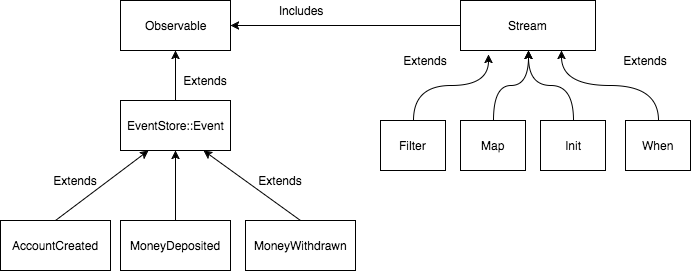
\includegraphics[scale=0.6]{img/class_diagram}
    \caption{Kuriamos bibliotekos klasių priklausomybių diagrama}
    \label{img:class_diagram}
\end{figure}

\textbf{Įvykių stebėsenos realizacija}

\lstinline|EventStore::Event| išplečia \lstinline|Observable| modulį ir šiuo atveju yra tema. Kiekvienas įvykio tipas sistemoje yra kuriamas paveldint \lstinline|EventStore::Event| klasę:

\begin{lstlisting}
class AccountCreated < EventStore::Event
end

# arba

AccountCreated = Class.new(EventStore::Event)
\end{lstlisting}

Kadangi tema yra klasė, o ne objektas (tokiu atveju programuotojui pačiam tektų informuoti stebėtojus), verta atskirai panagrinėti \lstinline|EventStore::Event| klasės objekto metodą \lstinline|emit|:

\begin{lstlisting}
def emit
  self.class.changed
  self.class.notify_observers(self.to_h)
end
\end{lstlisting}

Išplečiant klasę \lstinline|Observable| moduliu, pastarosios metodai yra pridedami klasei, o ne tos klasės objektui. Čia galima panaudoti introspekciją ir sužinoti kokio tipo objektui metodas yra kviečiamas. Taip informuojami visi stebėtojai, kurie prenumeruoja šią temą. Šis metodas yra iškviečiamas iškart po to kai įvykis būna įrašytas į duomenų saugyklą naudojantis anksčiau minėtu įvykių publikavimo mechanizmu. Galime pažvelgti į klasės \lstinline|EventRepository|, atsakingos už įvykių publikavimą, metodą \lstinline|create|:

\begin{lstlisting}
def create(event, stream_name)
  data = event.to_h.merge!(stream: stream_name)
  adapter.create(data)

  # Notify observers of new event
  event.emit if event.respond_to?(:emit)

  event
end
\end{lstlisting}

Kai tik įvykis išsaugomas duomenų saugykloje, visi įvykio prenumeratoriai yra informuojami apie naują įvykį sistemoje.

\textbf{Skaitymo modelio kūrimo aprašo realizacija}

Skaitymo modelis yra kuriamas pasinaudojant duomenų srautais. Inicializuojant duomenų srautą \lstinline|Stream.new(*sources)|, konstruktoriuje apibrėžiami prenumeruojami įvykiai:

\begin{lstlisting}
sources.each { source.add_observer(self) }
\end{lstlisting}

Srautas geba pats pasirūpinti, jog būtų informuotas apie naujus įvykius sistemoje.

Srautas taip pat realizuoja svarbų metodą \lstinline|update|, kuris yra visada iškviečiamas gavus naują įvykį.

Kiekvienas reaktyvus operatorius yra kuriamas labai panašiai, todėl pateiksime tik porą operatorių realizaciją:

\begin{lstlisting}
def filter(blk)
  Filter.new(self, blk)
end

def when(event_type, blk)
  When.new(self, event_type, blk)
end
#...
\end{lstlisting}

Grąžinama nauja atitinkama klasė, kuri paveldi \lstinline|Stream| srautą. Verta pastebėti, jog perduodamas ir pradinis srautas. Taigi srautas \lstinline|Stream| tuo pačiu metu gali būti ir stebėtojas, ir tema.

\textbf{Kuriamo skaitymo modelio tipo operatorius}

Norint išsaugoti tarpinę skaitymo modelio būseną duomenų saugykloje, reikia žinoti skaitymo modelio tipą bei jo pirminį raktą.

\lstinline|as_persistent_type(resource_type, unique_resource_identifier)| yra srauto metodas, kuris įsimena kuriamo skaitymo modelio tipą bei jo pirminį raktą. Naudojant reaktyvius operatorius, modelio tipas ir pirminis raktas yra automatiškai perduodami reaktyvaus operatoriaus srautui. Bendruoju atveju, pirminis raktas gali būti nuspėtas. Tarkime, jeigu kuriamas vartotojo sąskaitos skaitymo modelis \lstinline|Account|, pirminis raktas greičiausiai bus \lstinline|account_id|. Kartais gali atsirasti noras kurti sudėtingesnius skaitymo modelio vaizdus. Tarkime, programos vartotojas gali turėti kelias sąskaitas. Tokius atveju pirminis raktas turėtų būti pora \lstinline|user_id, account_id| - vartotojo kodas ir sąskaitos kodas. Norint sukurti tokį skaitymo modelį, užtektų kuriamo skaitymo modelio aprašo srautui iškviesti \lstinline|as_persistent_type(Account, [:account_id, :user_id])|. Pirminio rakto sudedamųjų dalių tvarka šiuo atveju nesvarbi. Metodas grąžina pasinaudoja metodų apjungimo principu, tai yra grąžina objektą, kuriam buvo iškviestas.

Įprastai programuotojas turi apsirašyti aktyvaus įrašo modelį pats \lstinline|class Account < ActiveRecord::Base; end|. Tačiau čia gali pasitarnauti meta programavimas \cite{Olsen:2007:DPR:1349728}, kuris leidžia programuotojams būti produktyvesniems generuojant dalį kodo. Šiuo atveju biblioteka leidžia paduoti ne tik jau aprašytą aktyvaus įrašo tipą, bet priima tiek eilutės, tiek simbolio tipą ir gali dinamiškai paveldėti aktyvaus įrašo bazinį tipą panaudojant refleksija:

\begin{lstlisting}
@resource_type =
  if defined_stream_type.is_a? String
    Object.const_set(dynamic_name, Class.new(ActiveRecord::Base))
  elsif defined_stream_type.is_a? Symbol
    Object.const_set(defined_stream_type.to_s.capitalize, Class.new(ActiveRecord::Base))
  else
    defined_stream_type
  end
\end{lstlisting}

\textbf{Filtravimo operatorius}

Filtravimo operatorius \lstinline|filter| priima predikatą, tai yra tam tikrą sąlygą. Jeigu ši sąlyga yra teisinga, įvykis yra perduodamas toliau visiem jo prenumeratoriams. Šis funkcionalumas realizuojamas pasinaudojant objektinio programavimo sąvybe polimorfizmu. Tėvinės klasės metodas \lstinline|update| yra perrašomas ir pakeitimai perduodami tik tada kai sąlyga yra išpildyta:

\begin{lstlisting}
class Filter < Stream
  def initialize(source, blk)
    @resource_type = source.resource_type
    @unique_resource_identifier = source.unique_resource_identifier
    @block = blk
    source.add_observer(self)
  end

  def update(event)
    occur(event) if @block.call(event)
  end
end
\end{lstlisting}

Galime panagrinėti šio reaktyvaus operatoriaus panaudojimo atvejį. Tarkime vartotojas sistemoje gali tiek nusipirkti prekę, tiek užsisakyti, jog prekė būtų pagaminta pagal užsakymą. Gali kilti noras konstruoti skaitymo modelį, apjungiantį juos abu bei turint papildomų sąlygų. Pavyzdžiui vartotojui gali būti suteikiami kreditai už sėkmingą pirkimą tik tada, kai:

\begin{itemize}
  \item Pirkinio vertė yra didesnė nei 100 eurų.
  \item Specialaus užsakymo vertė yra daugiau nei 50 eurų.
\end{itemize}

Tokį duomenų srautą galima konstruoti panaudojant reaktyvų filtravimo operatorių \lstinline|filter| kaip:

\begin{lstlisting}
  product_orders_eligible_for_bonus =
    Stream.new(ProductPurchased).
                filter( -> (event) event[:data][:price_paid] > 100)

  job_orders_eligible_for_bonus =
    Stream.new(JobOrderPurchased).
               .filter( -> (event) event[:data][:price_paid] > 50)
\end{lstlisting}

\textbf{Srautų sujungimo operatorius}

Apibrėžiant filtravimo operatorių, buvo sukurti 2 srautai, kurie yra filtruojami skirtingi. Norėdami pritaikyti bendrus veiksmus jiems, turime turėti galimybę juos sujungti. Šių filtruotų srautų sujungimo operatorius \lstinline|merge| atrodytų kaip:

\begin{lstlisting}
  merged_stream = product_orders_eligible_for_bonus.merge(job_orders_eligible_for_bonus)
\end{lstlisting}

Metodo \lstinline|merge| realizacija yra naujo srauto sukūrimas, panaudojant 2 srautus:

\begin{lstlisting}
def merge(another_stream)
  Stream.new(self, another_stream)
end
\end{lstlisting}

\textbf{Pradinės reikšmės operatorius}

\lstinline|init| metodas veikia kaip inicializatorius. Jeigu skaitymo modelis dar nėra saugomas duomenų saugykloje, sukuriant įrašą bus nustatoma pradinės įrašo reikšmės. Šiuo atveju sąskaitos balansas bus 0. Metodas priima \lstinline|lambda| funkciją, kuri bus iškviesta inicializavimo metu.

\begin{lstlisting}
def update(event)
  check_resource_type_presence

  entity_id_hash = extract_entity_id(event)

  if !@resource_type.where(entity_id_hash).exists?
    resource = @resource_type.new(event[:data])
    @block.call(resource)
    resource.save!
  end

  occur(event)
end
\end{lstlisting}

Čia \lstinline|update| metodas yra iškviečiamas kiekvieną kartą, kai duomenų srautas gauna naują įvykį, o stebėtojas jį prenumeruoja. \lstinline|Init| tipo srautas saugo informaciją apie kuriamą skaitymo modelio tipą, todėl iš gauto įvykio gali išgauti pirminio rakto informaciją. Jeigu toks skaitymo modelis dar nėra sukurtas sistemoje, naujas įrašas yra sukonstruojamas, pritaikoma būsenos keitimo funkcija ir programos tarpinė būsena yra išsaugoma duomenų saugykloje. Įvykis visada perduodamas toliau visiems prenumeratoriams.

\textbf{Tipo atitikimo operatorius}

Operatorių \lstinline|when(event_type, blk)| galima vadinti tipo atitikimo operatoriumi. Perduodamas \lstinline|lambda| blokas bus iškviestas tik tada kai sistemoje įvykusio įvykio tipas bus toks, koks yra apibrėžtas.

Jeigu tipai atitinka ir skaitymo modelio tarpinė būsena dar nėra saugoma duomenų saugykloje, šio operatoriaus realizacija yra identiška \lstinline|init| operatoriaus realizacijai.

Jeigu tipai atitinka ir skaitymo modelio tarpinė būsena jau yra saugoma duomenų saugykloje, būsena užklausiama, modifikuojama panaudojus būsenos keitimo funkciją, o gautas tarpinis rezultatas išsaugomas duomenų saugykloje:

\begin{lstlisting}
resource = @resource_type.where(entity_id_hash).first
@block.call(resource)
resource.save!
\end{lstlisting}

\textbf{Iteratoriaus operatorius}

Kartais gali vertėti klausytis kelių įvykių šaltinių ir jiems pritaikyti bendras operacijas. Tarkime norime atnaujinti informaciją paieškos duomenų saugykloje, kai pasikeičia kokia nors svarbi informacija apie produktą. Tokį funkcionalumą, galėtume išreikšti kaip:

\begin{lstlisting}[]
  Stream.new(ProductImageUploaded, ProductInformationChanged)
      .as_persistent_type(Product)
      .each( -> (state, event) state.reindex )
\end{lstlisting}

Iteratoriaus operatoriaus \lstinline|each| realizacija yra identiška tipo atitikimo operatoriui. Vienintelis skirtumas, jog būsenos keitimo funkcija yra pritaikoma visems prenumeruojamiems įvykiams.

\textbf{Skirtingi būdai struktūrizuoti skaitymo modelio aprašą}

Iš esmės \lstinline|lambda| blokas yra vykdomas, kai jam iškviečiamas \lstinline|call| metodas. Kadangi aprašyti operatoriai priima \lstinline|lambda| bloką kaip parametrą, esti papildomi būdai perduoti juos.

Galima apsirašyti kintamąjį:

\begin{lstlisting}
  variable = -> (event) { }
\end{lstlisting}

Taip pat galima apsirašyti klasę, kuri turi \lstinline|call| metodą:

\begin{lstlisting}
  class Denormalizers::ReadModelType::Event
    def call(state, event)
      # implementation
    end
  end
\end{lstlisting}

Lankstumas suteikia galimybę laisvai struktūrizuoti kodą, sutrumpinti skaitymo modelio kūrimo aprašą, kas gali pagerinti projekto priežiūrą, skaitomumą bei programuotojo produktyvumą.

\subsubsection{Apribojimai}

Sujungus reaktyvaus programavimo ir įvykių kaupimo principus ir sukūrus biblioteką, pastebėti tam tikri apribojimai, kuriuos verta paminėti:

\begin{itemize}
  \item Saugant tarpinę skaitymo modelio tipo būseną reikalingas ne tik tipas, bet ir to skaitymo modelio pirminis raktas. Šis identifikatorius paimamas iš prenumeruojamo įvykio nešamos informacijos. Dėl šio priežasties kiekvienas prenumeruojamas įvykis privalo turėti šią informaciją.
  \item Analizuojant įvykių kaupimo sistemų kūrimą bei teoriją, buvo pastebėta, jog kuriamas skaitymo modelis yra denormalizuotas, tai yra jis turi visą informaciją, reikalingą vaizdui pateikti. Dėl šios priežasties, biblioteka nepalaiko kelių skaitymo modelių, sujungtų išoriniais raktais, kūrimo.
  \item Srautas nėra baigtinis, operatorių funkcijos pritaikomos tik nutikus įvykiui, todėl neįmanoma užklausti pagal kintantį laiką. Pavyzdžiui, negalėtume sukurti tam tikro skaitymo modelio, kuris vaizduotų paskutinių 24h operacijas. Norint tikslumo, tam derėtų pasinaudoti įvykių saugyklos adapteriu \lstinline|EventRepository|, skaityti paskutinius įvykius sistemoje ir kurti laikiną skaitymo modelį nesinaudojant biblioteka.
  \item Sukurta biblioteka niekada nesunaikina tarpinės skaitymo modelio būsenos. Esant reikalui identifikuoti sunaikintą būseną, galima prenumeruoti naikinimo įvykį ir turėti tam tikrą \lstinline|status| identifikatorių, kuris pažymėtų skaitymo modelio būseną sistemoje. Pavyzdžiui, elektroninėje parduotuvėje gali tekti žinoti ar produktas pradedamas kelti, įkeltas, suspenduotas ar ištrintas.
\end{itemize}

\subsubsection{Pavyzdinis projektas panaudojantis aprašytą biblioteką}

Pilnas išeities kodas yra prieinamas skaitmeninėje laikmenoje, kuri yra pridėta prie darbo. Projekto aplanko pavadinimas yra \lstinline|cappuccino|. Pagrindinės nuorodos:

\begin{itemize}
  \item \lstinline|README.md| - aprašytos diegimo instrukcijos, testų paleidimo instrukcijos bei bibliotekos naudojimosi instrukcijos.
  \item \lstinline|app/lib/event_store| - bibliotekos failai, reikalingi įvykių publikavimui.
  \item \lstinline|app/lib/cappuccino| - bibliotekos failai, reikalingi kuriant skaitymo modelį panaudojant reaktyvųjį programavimą.
  \item \lstinline|spec/lib| - testai, užtikrinantys korektišką bibliotekos elgesį, tai yra validuojantys funkcionalumą.
\end{itemize}


